L'analyse lexicale vise à produire un flot de jetons qui pourront être analysés par l'analyseur syntaxique. Ces jetons sont des paires composées d'un type de jeton et de la valeur du lexème (par exemple, l'analyse du lexème \verb|12| va générer le jeton \verb|<NUMBER,12>| dans notre cas). Certains lexèmes peuvent générer des jetons qui n'ont pas de valeur (par exemple, le lexème \verb|(| va entraîner la génération du jeton \verb|<(>|).

Nous avons fait le choix d'utiliser l'outil Flex pour notre projet (cf.~\ref{Flex}).

\subsection{Jetons}
Notre analyseur lexical a dans un premier temps généré un nombre limité de jetons. Ainsi, en version 0.1, nous générions seulement 26 jetons différents (dont 5 jetons de littéraux), contre 40 jetons en version 1.0 (dont 7 jetons de littéraux). Ces jetons sont définis dans le code source bison (cf. listing~\ref{parser}) et leur valeur a un type C++ défini par la structure listing~\ref{struct-jeton}. Dans cette structure, l'attribut \verb|tok| correspond au type du jeton (défini par une énumération plus tard) tandis que l'attribut \verb|v| correspond à une valeur. En effet, notre langage ayant un typage dynamique, toutes les valeurs ont un type statique de type \verb|Value|. Ainsi, grâce au polymorphisme, le jeton aura une valeur qui pourra être de type dynamique \verb|Number|, \verb|String|, \verb|Boolean|, etc. tout en gardant un type statique de \verb|Value|. C'est lors de l'analyse sémantique (cf.~\ref{analyse-semantique}) que le type réel du jeton est analysé.

\begin{lstlisting}[label=struct-jeton,caption=Type des valeurs des jetons]
struct {
  stibbons::ValuePtr v;
  stibbons::TreePtr tr;
  int tok;
};
\end{lstlisting}

\subsection{Fonctionnement}
Par défaut, l'analyseur lexical généré par Flex utilise des variables globales et n'est pas réentrant. Dans l'optique d'obtenir un analyseur réentrant, nous avons utilisé l'option \verb|%option c++| et établit le modèle \ref{uml-lexer}.

\begin{figure}[h]
\centering
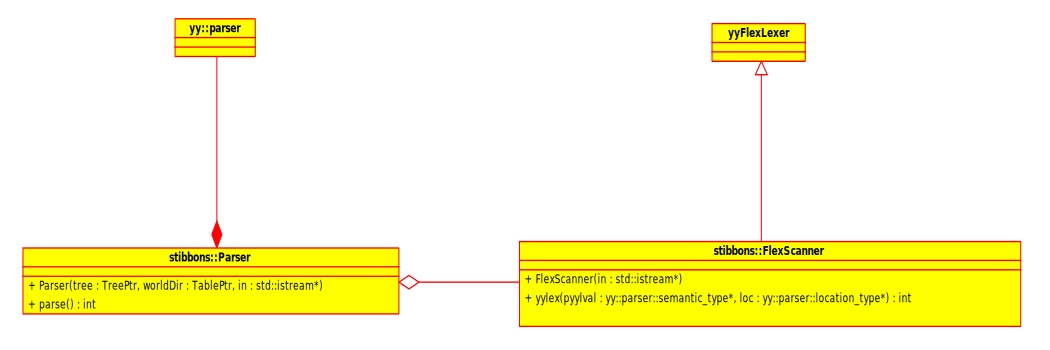
\includegraphics[scale=0.6]{doc/report/img/reentrant-parser}
\caption{\label{uml-lexer} UML des analyseurs lexical et syntaxique}
\end{figure}

Chaque appel à la méthode \verb|yylex()| de \verb|FlexScanner| génère un nouveau token à partir du flux d'entrée passé en paramètre lors de la construction de l'objet \verb|FlexScanner|. Cette méthode analyse le flux à partir des règles définies dans le fichier \verb|lexer.l+| (cf. listing~\ref{lexer}). Ainsi, les instructions définies pour chaque règle sont effectuées quand une chaîne de caractères correspondante à la règle est détectée. Ainsi, dans l'extrait \ref{lex-extrait}, lorsque l'analyseur détecte le caractère \verb|#| suivi d'une séquence de 3 ou 6 nombres hexadécimaux, l'appel au constructeur de \verb|Color(string)| est effectué. Ce dernier crée une couleur à partir d'une chaîne de caractère respectant les codes de couleur html.

\begin{lstlisting}[label=lex-extrait,caption=Exemple de séquence d'instructions lors de la détection d'une couleur]
#([a-f0-9]{6}|[a-f0-9]{3}) {
                           pyylval->v=make_shared<stibbons::Color>(yytext);
                           return yy::parser::token::COLOR;
                           }
\end{lstlisting}

De plus, l'instruction \verb|loc->step()| est effectuée au début de chaque appel à \verb|yylex()|, et permet de faire avancer la position actuelle de la longueur du lexème détecté, et l'instruction \verb|loc->lines()| est effectuée lors de la détection d'un retour à la ligne afin de faire avancer de \verb|n| lignes la position actuelle (avec \verb|n| le nombre de retour à la ligne détecté).
Les différentes règles flex peuvent être consultées au listing \ref{lexer}, ou de façon plus lisible dans l'annexe \ref{flex-rail}.
